\section{Implementación y control de versiones}

\subsection{Introducción}

\quad En esta parte se presentan las diferentes implementaciones necesarias, así como un control de versiones de la aplicación en la que se desmenuzan las diferentes versiones. \\

\quad Llevar un control de versiones es esencial como desarrollador, por lo que para este fin se utiliza la página \textit{github}, y como herramienta secundaria para la gestión del repositorio, la herramienta \textit{GitKraken}. Para el desarrollo de esta aplicación se ha seguido el paradigma de \textit{GitFlow} a la hora del control de versiones con el repositorio.\\

\subsection{Control de versiones}

\quad A continuación, se presenta el árbol de desarrollo de la aplicación en las que se ve un resumen de las modificaciones:

\begin{figure}[htb]
	\centering
	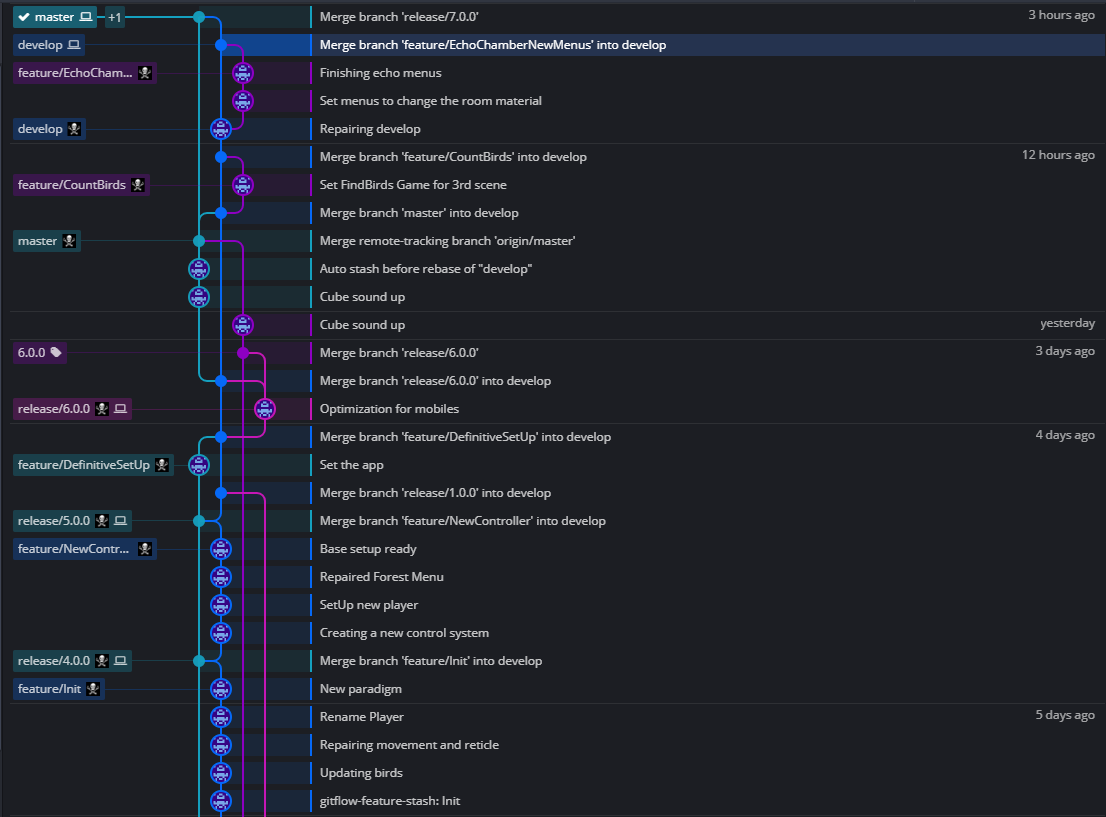
\includegraphics[width=0.8\textwidth]{./imagenes/git-tree1}
	\caption{Parte superior del gitTree}
\end{figure}
\FloatBarrier

\begin{figure}[htb]
	\centering
	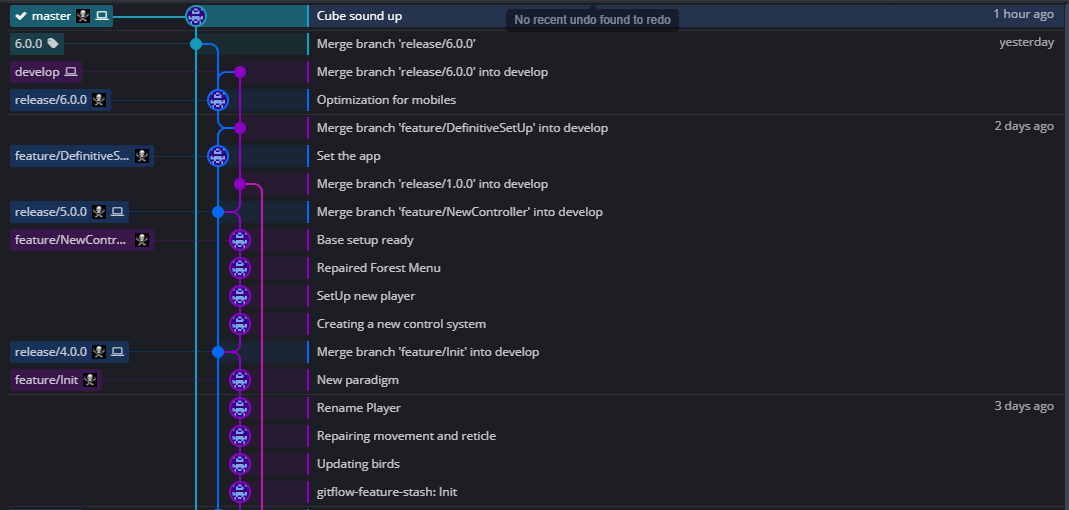
\includegraphics[width=0.8\textwidth]{./imagenes/git-tree2}
	\caption{Parte inferior del gitTree}
\end{figure}
\FloatBarrier

\subsubsection{Cambios orgánicos en el planteamiento de la aplicación}

\quad El desarrollo de una aplicación no es ni mucho menos algo estático que sigue estrictamente los pasos definidos al inicio de éste durante la planificación. Un buen desarrollo debe saber adaptarse a requisitos que pudieron no tenerse en un principio.\\

\quad Este es el caso de la aplicación aquí presentada, de forma que me dispongo a enumerar unos cuantos cambios que surgieron a lo largo del desarrollo y que merecen ser resaltados por encima de los demás:

\begin{itemize}
	\item En la versión 5.0.0, desecho un control del movimiento del personaje basado en mando por un control basado únicamente en los que el cardboard nos presenta, pasando el botón de pantalla a haber que el personaje se mueva hacia adelante, y las interacciones con elementos de las escenas presentadas con un cargador de tiempo. Este cambio surge ante el planteamiento de  facilitar el uso para el usuario, al no depender de otro dispositivo externo, en este caso un mando.
	\item En la versión 6.0.0 la retícula de carga pasa a ser la propia retícula puntero que utiliza. Esto se realiza con la idea de evitar que la superposición de ambas retículas pueda marear al usaron cuando la de carga entra en escena.
	\item En la versión 6.0.0 se aplica \textit{Oclussion Culling} en la escena del bosque. Esto se hace para reducir su carga y así maximizar los frames de la escena.
\end{itemize}

\subsection{Implementación general: setUp de la aplicación}

\quad El trabajo de esta aplicación se ha desarrollado con Unity 2018.4.6f1. Esto se ha hecho así debido a que el hub de Unity determinaba que esta era la última versión estable de la aplicación en el momento del inicio de la programación de este proyecto.\\

\quad Deberemos configurar también la sdk para que Unity pueda trabajar. Normalmente si ya se tiene la sdk de android instalada, Unity la reconocerá sin necesidad de añadirla manualmente.\\

\quad Debemos tener en cuenta que, en "Edit>Project Settings", debemos activar la casilla \textit{Virtual Reality Supported} de XR Settings para android en el "Player", y fijar en la pestaña "Other Settings" el \textit{Minimum API Leve} a nivel 19.\\

\subsubsection{Paquetes a descargar y assets gratuitos}

\quad Los paquetes que necesitaremos para poder utilizar la tecnología necesaria en Unity son:

\begin{itemize}
	\item ResonaceAudioForUnity\_<versión\_deseada>.unitypackage \cite{DResonance}
	\item GoogleVRForUnity\_<versión\_deseada>.unitypackage \cite{DGvr}
\end{itemize}

\quad El paquete GoogleVR es un set de utilidades desarrolladas por google para facilitar el desarrollo de una aplicación con realidad virtual que además tiene versión para varios motores.\\

\quad El paquete Resonance es un set de herramientas con los algoritmos pertinentes para poder simular los distintos aspectos de un sonido envolvente, con distintos efecto, percepción de profundidad (conocido como sonido 3D) y sonido 8D.\\

\quad En la documentación hay un enlace para poder acceder a todas las características aplicadas a Unity para ambos paquetes \cite{Gvr} \cite{Resonance}.\\


\quad Para instalar un paquete descargado, solo habrá que introducir el paquete manualmente desde la pestaña \textit{Assets>Import Package>Custom Package}.\\

\quad Por otra parte, los assests gratuitos sacados de la store de Unity son los siguiente:

\begin{itemize}
	\item Fantasy Forest
	\item Hand Painted Forest Lite
	\item Living Birds
\end{itemize}

\quad \textit{Fantasy Forest} ha sido utilizado para extraer el modelaje de los árboles y la textura 2D para la hierba. La aplicación de los árboles en un terreno, así como de la hierba se hace siguiendo el procedimiento standard de Unity.

\begin{figure}[htb]
	\centering
	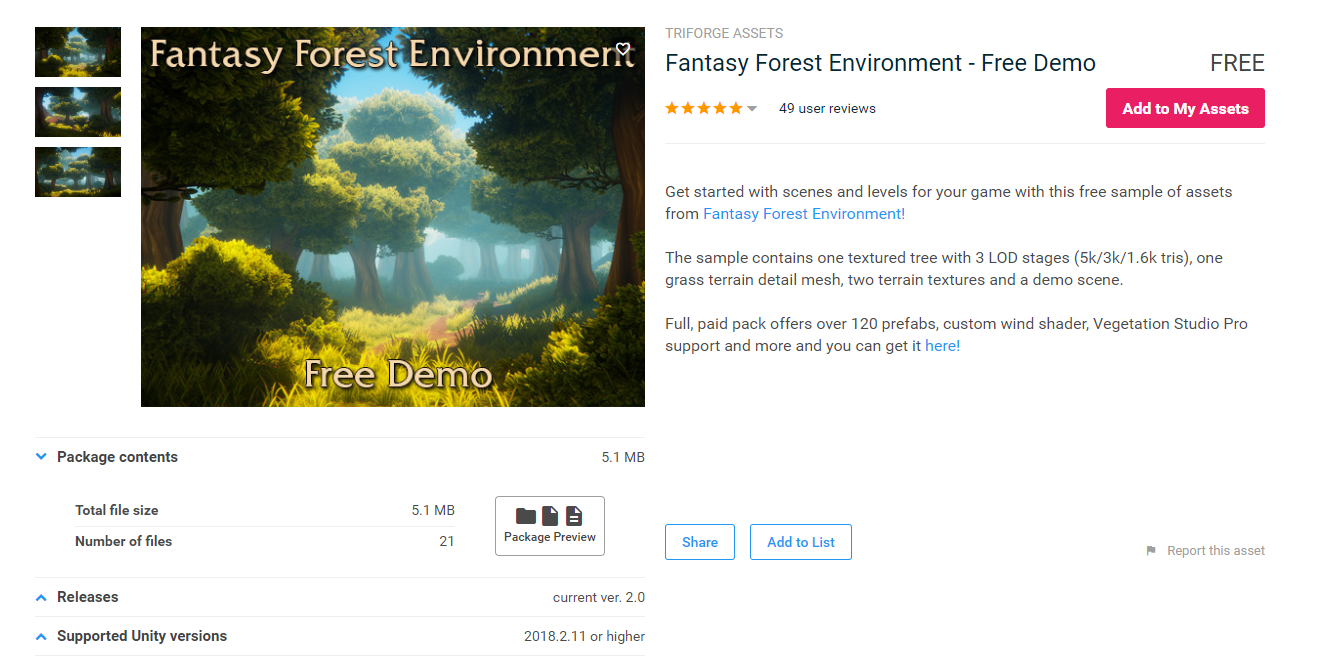
\includegraphics[width=0.7\textwidth]{./imagenes/fantasyForest}
	\caption{Fantasy Forest}
\end{figure}
\FloatBarrier

\quad \textit{ Hand Painted Forest Lite} ha sido descargado exclusivamente por el modelado de las estatuas, las cuáles han sido integradas al terreno en el que el jugador se sitúa.

\begin{figure}[htb]
	\centering
	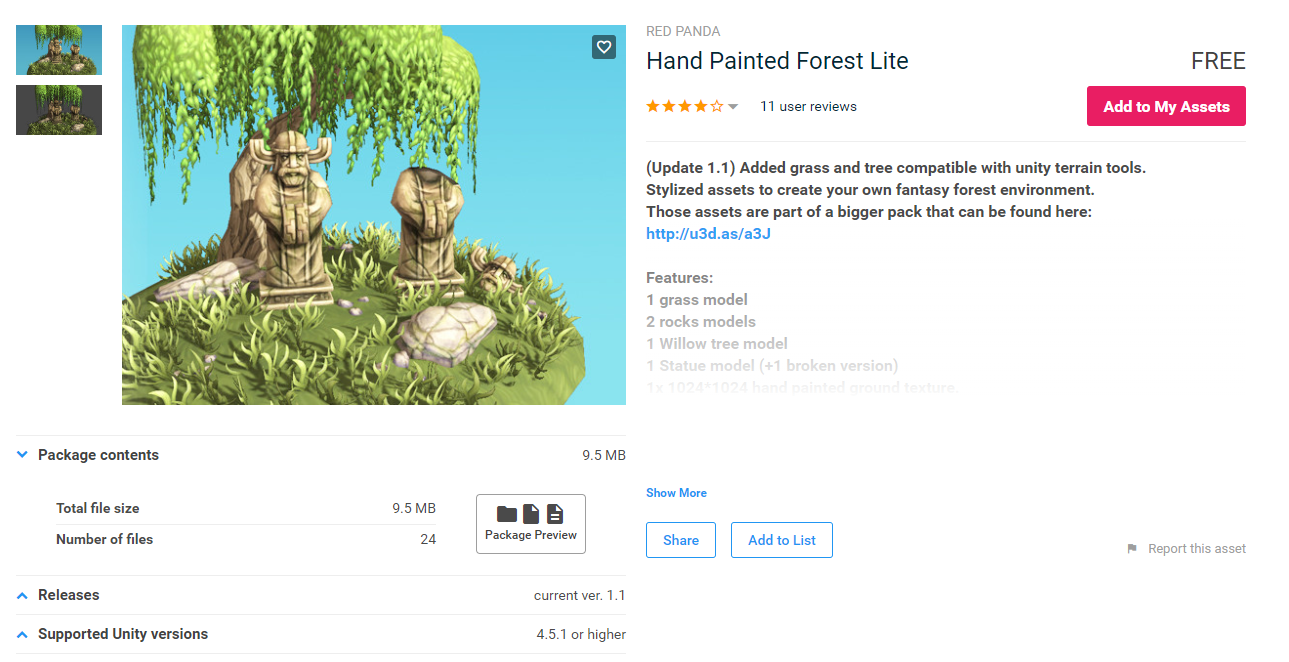
\includegraphics[width=0.7\textwidth]{./imagenes/handPaintedForest}
	\caption{Hand Painted Forest Lite}
\end{figure}
\FloatBarrier

\quad \textit{Living Birds} posee los modelados y animaciones de los pájaros, además de un sistema para hacer que los pájaros se generarán automáticamente para simular un entorno orgánico. en el momento en el que se utilizó este asset, lo único implementado fueron los modelajes con sus animaciones, ya que la mayoría de script asociados a la generación automática estaban vacíos, o directamente no existían, por lo que parte del desarrollo se dedicó a rehacer gran parte de este asset.

\begin{figure}[htb]
	\centering
	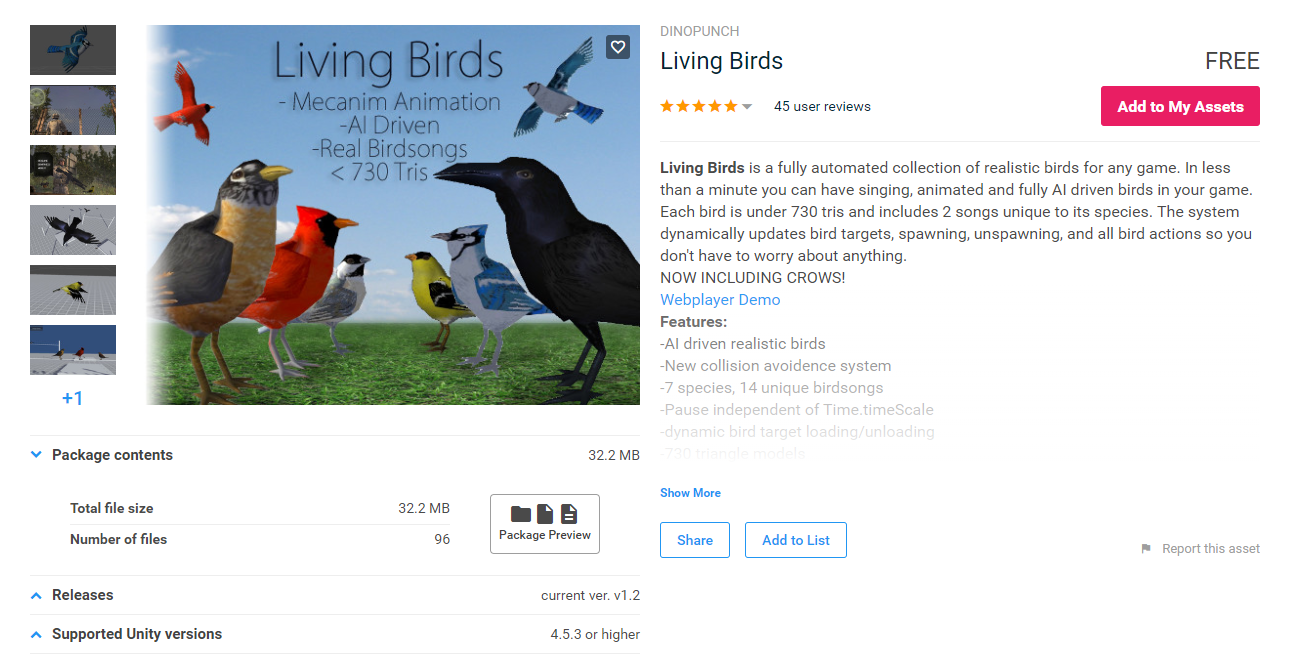
\includegraphics[width=0.7\textwidth]{./imagenes/livingBirds}
	\caption{Living Birds}
\end{figure}
\FloatBarrier

\subsection{Jugador}

\quad El jugador estará formado por un GameObject llamado \textit{RealPlayer} que contendrá la "MainCamera". Se introducirá como hijo de ésta el prefab \textit{GvrReticlePointer} que pondrá en el jugador la retícula que utilizaremos para las interacciones. Hay una serie de cambios en la retícula que se explican en el siguiente subapartado.\\

\begin{figure}[htb]
	\centering
	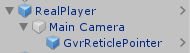
\includegraphics[width=0.5\textwidth]{./imagenes/player}
	\caption{Aspecto del Jugador en el árbol de escena}
\end{figure}
\FloatBarrier

\subsubsection{Controles de movimiento}

\quad Se ha implementado para el movimiento que cuando se hace click en la pantalla, el jugador se mueve. Esto se consigue añadiendo un script de C\# a \textit{RealPlayer} que contendrá el siguiente código:

\lstset{language=[sharp]C, breaklines=true, basicstyle=\footnotesize}
\begin{lstlisting}[frame=single, caption={PlayerWalk.cs}]
using System.Collections;
using System.Collections.Generic;
using UnityEngine;

public class PlayerWalk : MonoBehaviour
{
    public int playerSpeed;

    // Update is called once per frame
    void Update()
    {
        if (Input.GetButton("Fire1")) {
            transform.position = transform.position + Camera.main.transform.forward * playerSpeed * Time.deltaTime;
        }
    }
}

\end{lstlisting}

\subsubsection{Control de cámara en VR}

\quad Simplemente se añadirá al árbol de escena el prefab de GoogleVR \textit{GvrEditorEmulator}, que en ordenador proporciona una vista normal mientras que al instalar la apk en un dispositivo, este mostrará la pantalla dividida y adaptada para ser utilizada en un dispositivo de visionado como las \textit{cardboard}.\\

\quad El control simulado en el PC se utiliza de la siguiente manera:
\begin{itemize}
	\item \textit{Alt + move} mouse para rotar sobre uno mismo y cambiar la dirección a la que se orienta el jugador
	\item \textit{Ctrl + move} mouse para rotar sobre el eje que sale desde el jugador hacia adelante
\end{itemize}

\quad No voy a entrar en detalles con el código del objeto en cuestión ya que no es código propio.\\

\subsubsection{Retícula}

\quad La retícula que viene por defecto en unity no será necesaria en el caso presentado, pues es mejor y más eficiente utilizar el script \textit{GvrPointerPhysicsRaycaster.cs}, adjunto con el paquete de GoogleVR.\\

\quad La retícula es el medio para interactuar con el medio, pero no interesa que se active automáticamente, si no que será preciso que haya un tiempo de espera para que el usuario decida si se va a llevar a cabo esta interacción o si por el contrario desea cancelarla.\\

\quad Con motivo de ello, se aprovechará la capacidad de la retícula de google de ampliarse en una interacción (efecto producido con el prefab \textit{GvrEventSystem}.) y se modificará el ángulo mostrado en pantalla de ésta el cual se irá modificando, convirtiéndola así en una barra de carga circular. Para esto se requieren las siguientes modificaciones en el shader \cite{ShadersTut} de Google:

\begin{itemize}
	\item Añadir la propiedad Angle
	\item Añadir el float que la representará
	\item Sustituir la función \textit{vert} para para que tenga en cuenta esta nueva propiedad en el shader
\end{itemize}
\FloatBarrier

\quad A continuación se adjunta el resultado final para ver como debe quedar el código:

\lstset{language=[sharp]C, breaklines=true, basicstyle=\footnotesize}
\begin{lstlisting}[frame=single, caption={GvrReticleShader.shader}]
// Copyright 2015 Google Inc. All rights reserved.
//
// Licensed under the Apache License, Version 2.0 (the "License");
// you may not use this file except in compliance with the License.
// You may obtain a copy of the License at
//
// http://www.apache.org/licenses/LICENSE-2.0
//
// Unless required by applicable law or agreed to in writing, software
// distributed under the License is distributed on an "AS IS" BASIS,
// WITHOUT WARRANTIES OR CONDITIONS OF ANY KIND, either express or implied.
// See the License for the specific language governing permissions and
// limitations under the License.

// Trololo

Shader "GoogleVR/Reticle" {
Properties {
_Color ("Color", Color) = ( 1, 1, 1, 1 )
_InnerDiameter ("InnerDiameter", Range(0, 10.0)) = 1.5
_Angle("Angle", Range(0, 360)) = 180 // Propiedad con la que trabajaremos en el shader
_OuterDiameter ("OuterDiameter", Range(0.00872665, 10.0)) = 2.0
_DistanceInMeters ("DistanceInMeters", Range(0.0, 100.0)) = 2.0
}

SubShader {
Tags { "Queue"="Overlay" "IgnoreProjector"="True" "RenderType"="Transparent" }
Pass {
Blend SrcAlpha OneMinusSrcAlpha, OneMinusDstAlpha One
AlphaTest Off
Cull Back
Lighting Off
ZWrite Off
ZTest Always

Fog { Mode Off }
CGPROGRAM

#pragma vertex vert
#pragma fragment frag

#include "UnityCG.cginc"

uniform float4 _Color;
uniform float _InnerDiameter;
uniform float _OuterDiameter;
uniform float _DistanceInMeters;
uniform float _Angle; // Variable con la que trabajar 

struct vertexInput {
float4 vertex : POSITION;
};

struct fragmentInput{
float4 position : SV_POSITION;
};

/* fragmentInput vert(vertexInput i) {
float scale = lerp(_OuterDiameter, _InnerDiameter, i.vertex.z);

float3 vert_out = float3(i.vertex.x * scale, i.vertex.y * scale, _DistanceInMeters);

fragmentInput o;
o.position = UnityObjectToClipPos (vert_out);
return o;
}
*/


// Nueva version del metodo vert 
// que tiene en cuenta elangulo a la hora del dibujado
fragmentInput vert(vertexInput i) {
	 fragmentInput o;
	 if (_DistanceInMeters < 20) {
		 // 180* = 2.9
		 // limit = - (a - 180) * 2.9/180
		 float limit = -(_Angle - 180) * 0.0161111111;
		 float3 vert_out = float3(0, 0, _DistanceInMeters);
		 float a = -atan2(i.vertex.x, i.vertex.y);
		 if (a >= limit) {
			 float scale = lerp(_OuterDiameter, _InnerDiameter, i.vertex.z);
			 vert_out = float3(i.vertex.x * scale, i.vertex.y * scale, _DistanceInMeters);
		 }
		 o.position = UnityObjectToClipPos(vert_out);
	 }
	 return o;
}

fixed4 frag(fragmentInput i) : SV_Target {
fixed4 ret = _Color;
return ret;
}

ENDCG
}
}
}

\end{lstlisting}

\subsubsubsection{Interacción de la retícula}

\quad Ahora entra en juego como conseguir la interacción con el objeto. Para ello se requieren dos pasos muy importantes: \\

\begin{itemize}
	\item Añadir al objeto un \textit{EventTrigger} que trabajará cuando el puntero entre dentro del área que ocupa el objeto y cuando salga.
	\item Añadir un script al objeto que en este caso se ha llamado \textit{GVRButton.cs}.
\end{itemize}
\FloatBarrier

\quad Lo primero debe hacerse para determinar las funciones GvrOn y GvrOff que determinarán el comportamiento ante la entrada y la salida del objeto. El segundo determina la acción que se llevará a cabo a partir de que termine el evento de entrada, que en este caso que la barra de carga termine de llenarse.\\

\quad Se adjuntan seguidamente es aspecto de un objeto que posee estas cualidades y el código asociado a \textit{GVRButton.cs}.\\

\lstset{language=[sharp]C, breaklines=true, basicstyle=\footnotesize}
\begin{lstlisting}[frame=single, caption={GVRButton.cs}]
using System.Collections;
using System.Collections.Generic;
using UnityEngine;
using UnityEngine.UI;
using UnityEngine.Events;

public class GVRButton : MonoBehaviour
{
    GameObject pointer;
    public UnityEvent GVRClick;
    public float totalTime = 2;
    bool gvrStatus;
    public float gvrTimer;
    Renderer rend;
    float angle;
    bool counted;

    private void Start()
    {
        pointer = GameObject.FindWithTag("gvrpointer"); 	// Busqueda del puntero con elq ue se va a trabajar
        rend = pointer.GetComponent<Renderer>();		// Extraccion del renderer del puntero
        counted = false;						// Filtro para el conteo de parajaros en el bosque
    }

    // Update is called once per frame
    void Update()
    {
        if (gvrStatus)
        {
            gvrTimer += Time.deltaTime;			// Calculo de la fraccion de tiempo de la carga en la que se esta trabajando
            angle = gvrTimer / totalTime * 360;		// Calculo de la fraccion de arco a dibujar
            rend.material.SetFloat("_Angle", angle);	// Cambiar la variable angulo de la reticula
        }

        if (gvrTimer > totalTime)
        {
            GVRClick.Invoke();					// Efectuar un click
            gvrStatus = false;					// Determinar que se ha terminado la ejecucion
	 GvrOff();
        }
    }

// Metodo de inicio de interaccion de la reticula 
    public void GvrOn()
    {
        gvrStatus = true;
    }

// Metodo de finalizacion de interaccion de la reticula
    public void GvrOff()
    {
        gvrStatus = false;
        gvrTimer = 0;
        rend.material.SetFloat("_Angle", 360f);
    }

// Metodo para marcar los pajaros vistos en el cartel del bosque
    public void checkBird(string bird)
    {
        if (!counted)
        {
            GameObject.FindWithTag(bird).GetComponent<Text>().text = "OK";
            counted = true;
        }
    }
}

\end{lstlisting}

\begin{figure}[htb]
	\centering
	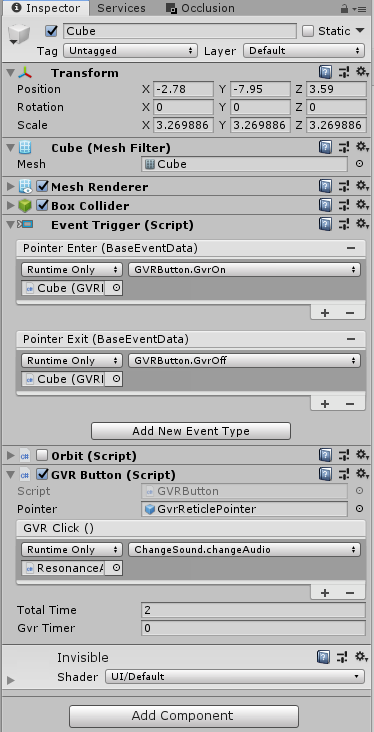
\includegraphics[width=0.8\textwidth]{./imagenes/cube}
	\caption{Cubo con interacciones}
\end{figure}
\FloatBarrier

\quad En el código se muestra como acceder al shader y modificar el ángulo que creamos en el apartado anterior dentro de la función update.\\

\subsubsection{Aplicar sonido 8D a un objeto}

\quad Esta parte se soluciona rápidamente añadiendo los dos siguientes elementos al objeto emisor de sonido y a la mainCamera:\\

\begin{itemize}
	\item El script \textit{ResonanceAudioListener.cs} a la main camera de la escena.
	\item El prefab\textit{ResonanceAudioSource} al objeto que hará de emisor.
\end{itemize}

\quad Es importante añadir el audio que queremos que se reproduzca en la propiedad \textit{Audio Source} para que los scripts puedan trabajar.

\begin{figure}[htb]
	\centering
	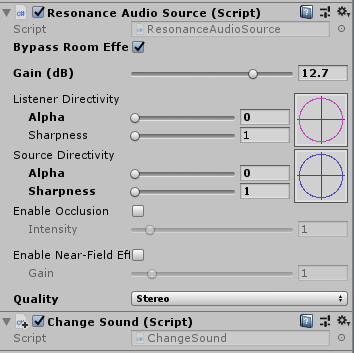
\includegraphics[width=0.6\textwidth]{./imagenes/audiosource}
	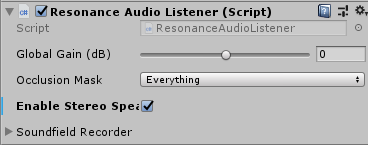
\includegraphics[width=0.6\textwidth]{./imagenes/audiolistener}
	\caption{Script ResonaceAudioSource y ResonanceAudioListener en el Inspector}
\end{figure}
\FloatBarrier

\subsection{Implementación por escenas}

\quad Ahora analizaremos los detalles más importantes implementados por escena.\\
	\subsubsection{Escena Init}
		\subsubsubsection{Cubo para interactuar}

\quad Ya se ha hablado de el cubo de la primera escena que interactúa con el usuario cuando lo mira, pero tiene varias acciones que realizar en el momento de la interacción:

\begin{itemize}
	\item Cambiar el audio que se está reproduciendo durante la ejecución.
	\item Cambiar la escena en la que se encuentra el jugador.
	\item Cambiar el material del cubo para que se haga visible.
\end{itemize}

\quad La primera acción requiere que por nuestra parte creemos un script que active la subrutina que cambie en ejecución el audio reproducido. La segunda acción requiere que cuando se termine de reproducir el nuevo audio se cargue la siguiente escena. El siguiente código muestra cómo hacer ambas cosas desde la subrutina WaitFinish:\\

\lstset{language=[sharp]C, breaklines=true, basicstyle=\footnotesize}
\begin{lstlisting}[frame=single, caption={ChangeSound.cs}]
using System.Collections;
using System.Collections.Generic;
using UnityEngine;
using UnityEngine.SceneManagement;
using UnityEngine.Timeline;

public class ChangeSound : MonoBehaviour
{
    AudioSource myaudio;
    Material mymaterial;
    Renderer rend;

    public void changeAudio()
    {
        mymaterial = Resources.Load<Material>("RedMat");	// Busca el material por el que se va a cambiar
        rend = GetComponentInParent<Renderer>();		// Se obtiene el renderer del padre
        rend.enabled = true;						// Nos aseguramos de que este activo
        rend.sharedMaterial = mymaterial;				// Se cambia el material
        StartCoroutine(WaitFinish());				// Se llama a la subrutina que cambia el audio durante la ejecucion
    }


// Subrutina que espera a que un audio termine de reproducirse completamente para avanzar a la siguiente escena 
    IEnumerator WaitFinish()
    {
        myaudio = GetComponent<AudioSource>();			// Localiza el componente AudioSource de la fuente de sonido
        myaudio.clip = Resources.Load<AudioClip>("porfinteveo3");	// Cambia el audio reproducido por el foco de sonido
        myaudio.Play();							// Reproduce el nuevo audio
        yield return new WaitForSeconds(myaudio.clip.length);	// Espera la longitud del audio reproducido
        SceneManager.LoadScene("EcoChamber");			// Carga de la nueva escena
    }
}

\end{lstlisting}

\quad En el mismo código se incluye dentro de la función changeAudio el método para poder cambiar el material de un GameObject.\\

	\subsubsection{Escena Echo Chamber}
		\subsubsubsection{Aplicar eco}
\quad Dentro del GameObject que define la habitación se debe añadir el prefab ResonanceAudioRoom, modificando el tamaño de este para que se ajuste al tamaño de la habitación.

\begin{figure}[htb]
	\centering
	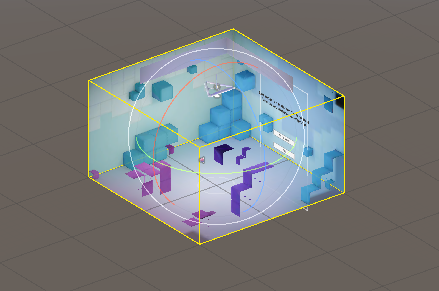
\includegraphics[width=0.55\textwidth]{./imagenes/echoroom}
	\caption{ResonanceAudioRoom ajustado a la habitación de la escena}
\end{figure}
\FloatBarrier

\quad Desde el script asociado al prefab, se pueden modificar los materiales que componen las diferentes caras del cubo que delimita el espacio que dispondrá de eco, así como las características del eco en cuestión (reflectividad, tiempo, ganancia en DB, brillo).

\begin{figure}[htb]
	\centering
	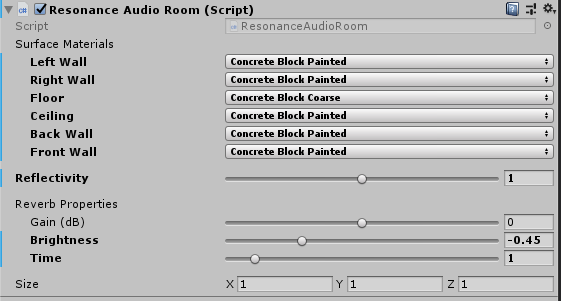
\includegraphics[width=0.8\textwidth]{./imagenes/audioroom}
	\caption{Script ResonaceAudioRoom}
\end{figure}
\FloatBarrier

		\subsubsubsection{Cambiar en escena los materiales de la habitación}

\quad En la aplicación se encuentran varios materiales implementados para los diferentes lados del cubo que delimita la zona. Para simplificarlo, en esta aplicación solo se han implementado una pequeña porción para demostrar un ejemplo de cambio de material dinámico de estos.\\

\quad La implementación de \textit{dropdown} ha sido llevada a cabo mediante el objeto suministrado por Unity. Debido a que no se dispone de una versión de pago para el desarrollo de esta aplicación, no se pueden tocar internamente el script que lo pone en funcionamiento, pero hay total libertad a la hora de añadir lo elementos que se requieran en la implementación.\\

\quad Siguiendo ese razonamiento, durante este desarrollo se han añadido un \textit{eventTrigger} y el script anteriormente mencionado \textit{GVRButton}, haciendo la configuración requerida para poder interactuar con los elementos internos del dropdown.\\

\begin{figure}[htb]
	\centering
	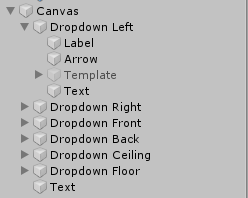
\includegraphics[width=0.5\textwidth]{./imagenes/dropdown}
	\caption{Dropdown en la jerarquía de escena}
\end{figure}
\FloatBarrier

\begin{figure}[htb]
	\centering
	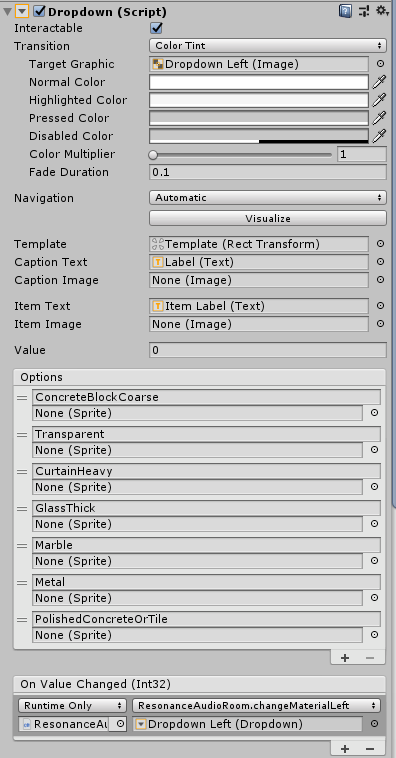
\includegraphics[width=0.8\textwidth]{./imagenes/dropDownScriptUnity}
	\caption{Script de un dropdown}
\end{figure}

\quad Como se puede apreciar, no hay problema a la hora de definir los elementos del desplegable, a los que se les asignará por defecto un valor entero en el orden en el que son añadidos.\\

\quad Para poder acceder al valor asignado, en la zona de \textit{OnValueChage} se ha añadido al elemento \textit{ResonanceAudioRoom} como GameObject, y se llama a una de las funciones que se montaran dentro de su propio código llamadas \textit{changeMaterialRight}, \textit{changeMaterialLeft}, \textit{changeMaterialFront}, \textit{changeMaterialBack}, \textit{changeMaterialCeiling} y \textit{changeMaterialFloor}.\\

\begin{figure}[htb]
	\centering
	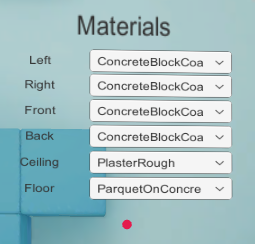
\includegraphics[width=0.8\textwidth]{./imagenes/materialMenu}
	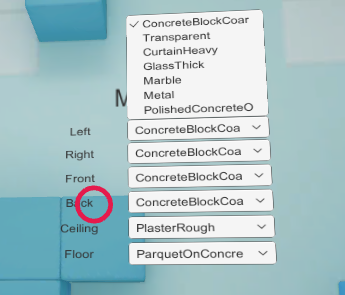
\includegraphics[width=0.8\textwidth]{./imagenes/materialMenuDeploy}
	\caption{Menú de cambio de material}
\end{figure}
\FloatBarrier

\quad La implementación de las seis funciones mencionadas es prácticamente la misma, ya que solo se varía la referencia al lado sobre el que se vana hacer las modificaciones.\\

\lstset{language=[sharp]C, breaklines=true, basicstyle=\footnotesize}
\begin{lstlisting}[frame=single, caption={Función changeMaterialLeft}]
...
public ResonanceAudioRoomManager.SurfaceMaterial rightWall =
	ResonanceAudioRoomManager.SurfaceMaterial.ConcreteBlockCoarse;
...
public void changeMaterialLeft(Dropdown mine) {
        int value = mine.value;	// Se obtiene el valor que tiene la opcion seleccionada del dropdown

        switch (value)			// Dependiendo del valor obtenido se el material con el que se cambiara 
        {
            case 0:
                leftWall = ResonanceAudioRoomManager.SurfaceMaterial.ConcreteBlockCoarse;
                break;
            case 1:
                leftWall = ResonanceAudioRoomManager.SurfaceMaterial.Transparent;
                break;
            case 2:
                leftWall = ResonanceAudioRoomManager.SurfaceMaterial.CurtainHeavy;
                break;
            case 3:
                leftWall = ResonanceAudioRoomManager.SurfaceMaterial.GlassThick;
                break;
            case 4:
                leftWall = ResonanceAudioRoomManager.SurfaceMaterial.Marble;
                break;
            case 5:
                leftWall = ResonanceAudioRoomManager.SurfaceMaterial.Metal;
                break;
            case 6:
                leftWall = ResonanceAudioRoomManager.SurfaceMaterial.PolishedConcreteOrTile;
                break;
            default:
                break;
        }
    }

\end{lstlisting}


		\subsubsubsection{Icosaedro el sonido}

\quad Respecto al icosaedro solo queda añadir la función que lo hace teleportarse cuando el evento entra en acción. Esta función se recoge en el siguiente código:\\

\lstset{language=[sharp]C, breaklines=true, basicstyle=\footnotesize}
\begin{lstlisting}[frame=single, caption={Teleporter.cs}]
using System.Collections;
using System.Collections.Generic;
using UnityEngine;

public class Teleporter : MonoBehaviour
{
    Vector3 destination; // Almacenara la posicion random
    RectTransform rt;
    
// Se cambia la posicion del icosaedro por una posicion random
    public void randomPlace()
    {
        destination = new Vector3(Random.Range(-8, 8), Random.Range(1, 8), Random.Range(-8, 8));
        rt = GetComponent<RectTransform>();
        rt.transform.localPosition = destination;
    }
}

\end{lstlisting}

	\subsubsection{Escena Forest}
		\subsubsubsection{Oclusion Culling}
\quad Occlusion Culling \cite{Culling} es una característica que desactiva el renderizado de objetos cuando actualmente no estén visibles por la cámara puesto que están oscurecidos (occluded) por otros objetos. Esto no sucede automáticamente en gráficas computacionales 3D ya que la mayoría de veces los objetos que están más lejos de la cámara son dibujados primero y los objetos más cercanos son dibujados encima de estos (esto se llama “overdraW”). El Occlusion Culling es diferente del Frustum Culling, ya que este solamente desactiva los renderers para objetos que están fuera del área visible de la cámara, pero no desactiva nada oculto de la vista por overdraw.\\

\quad Para que el culling funcione, los objetos que se deseen ver afectados por él deben tener la casilla Static activada. De esta forma evitamos que objetos que se mueven se vean afectados por la desaparición en el dibujado.\\

\begin{figure}[htb]
	\centering
	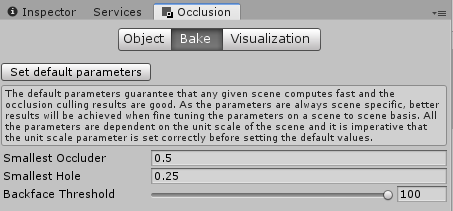
\includegraphics[width=0.8\textwidth]{./imagenes/cullingdata}
	\caption{Parámetros aplicados en la aplicación para el culling}
\end{figure}
\FloatBarrier

\begin{figure}[htb]
	\centering
	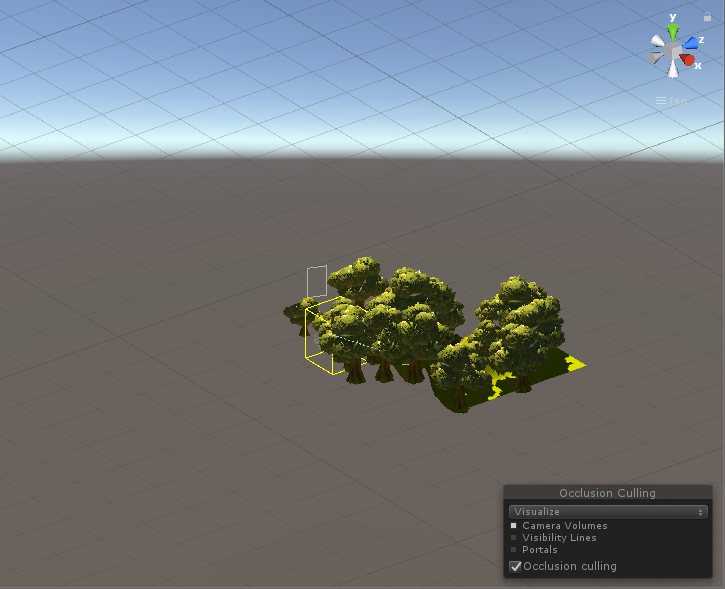
\includegraphics[width=0.40\textwidth]{./imagenes/culling1}
	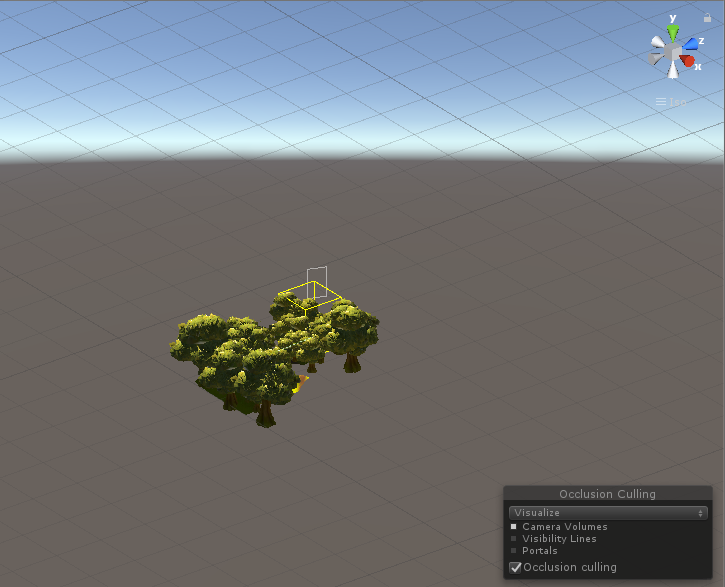
\includegraphics[width=0.40\textwidth]{./imagenes/culling2}
	\caption{Script ResonaceAudioRoom}
\end{figure}
\FloatBarrier

		\subsubsubsection{Pájaros y su búsqueda}

\quad El sonido en los pájaros se genera de la misma forma que en cualquier elemento con sonido (el cubo o el icosaedro), aunque presentan una pequeña diferencia. Donde encontremos dentro del script \textit{lb\_Bird.cs} una reproducción de uno de los cuatro audios que componen los sonidos del pájaro, se debe tener en cuenta que ahora el pájaro no contará con un AudioSource propio, si no que ese componente se encontrará dentro del objeto hijo ResonanceAudioSource que se le añadirá.\\

\quad Para poder acceder al componente de este objeto hijo, se debera cambiar la linea que hace el play por lo siguiente:\\

\lstset{language=[sharp]C, breaklines=true, basicstyle=\footnotesize}
\begin{lstlisting}[frame=single, caption={Ejemplo de cambio de audio para pájaro}]
	this.transform.Find("ResonanceAudioSource").gameObject.GetComponent<AudioSource>().PlayOneShot (song1,1);
\end{lstlisting}

\quad Deben hacerse cuatro cambios en el script \textit{lb\_Bird.cs}.\\

\quad Lo último a tener en cuenta en esta escena, es cambiar el shader de los materiales que componen la escena a \textit{Movile/Diffuse}. De esta forma se garantiza que el shader está optimizado para trabajar en un móvil.\\

\quad Ahora toca la implementación para poder interactuar con los distintos pájaros que aparecen en la escena, de forma que cuando interactuemos con dentro de la lista \textit{Most Wanted!!} situada encima del menú en el bosque, ésta chequee a ese ave en particular y la marque con un \textit{OK}.\\

\quad Con ese fin se ha escrito dentro del script GVRButton la función checkBird, a la cual se le pasa un string, el cual será el tag del texto que deberemos cambiar de vacío a "OK".\\

\begin{lstlisting}[frame=single, caption={función checkBird}]
// Metodo para marcar los pajaros vistos en el cartel del bosque
    public void checkBird(string bird)
    {
        if (!counted)
        {
            GameObject.FindWithTag(bird).GetComponent<Text>().text = "OK";
            counted = true;
        }
    }
\end{lstlisting}

\quad Es importante recordar que hay que modificar el prefab de cada pájaro que se quiera convertir en interactivo mediante los pasos que ya se explicaron con anterioridad.\\


\newpage





